
%(BEGIN_QUESTION)
% Copyright 2010, Tony R. Kuphaldt, released under the Creative Commons Attribution License (v 1.0)
% This means you may do almost anything with this work of mine, so long as you give me proper credit

\noindent
{\bf Programming Challenge -- Alarm event latch and history timers} 

\vskip 10pt

A normally-closed (NC) high-pressure sensing switch monitors fluid pressure in a chemical reactor vessel, opening its contacts if the pressure exceeds the trip point.  This triggers an alarm lamp to energize in the control room, and this lamp will latch in the ``on'' state until an operator resets it, even if the high-pressure condition ``clears'' and goes back to normal.  This is so the operators will know a high-pressure event occurred even if they were not in the control room to see it when it happened.  A PLC implements this latching function using retentive (``set'' and ``reset'') coils:

$$\includegraphics[width=15.5cm]{i02265x01.eps}$$

The system works well, but the operators want more.  If they arrive at the control room to see the alarm light on (latched), they want to know how long the high-pressure condition lasted and also how long it's been since the reactor pressure returned to normal.

\vskip 10pt

Add instructions to this PLC program to provide the desired timing functionality.

\vskip 20pt \vbox{\hrule \hbox{\strut \vrule{} {\bf Suggestions for Socratic discussion} \vrule} \hrule}

\begin{itemize}
\item{} Explain why the PLC program contact for the high-pressure switch is {\it normally-closed}, and how this information alone would be enough for us to determine that the high-pressure switch itself had NC contacts.
\item{} What type of timer instruction is best suited for the event duration timer, a {\it retentive} or a {\it non-retentive} timer?
\item{} How could a {\it counter} instruction be added to this PLC program to provide useful functionality?
\end{itemize}

\vfil 

\underbar{file i02265}
\eject
%(END_QUESTION)





%(BEGIN_ANSWER)


%(END_ANSWER)





%(BEGIN_NOTES)

I strongly recommend students save all their PLC programs for future reference, commenting them liberally and saving them with special filenames for easy searching at a later date!

\vskip 10pt

I also recommend presenting these programs as problems for students to work on in class for a short time period, then soliciting screenshot submissions from students (on flash drive, email, or some other electronic file transfer method) when that short time is up.  The purpose of this is to get students involved in PLC programming, and also to have them see other students' solutions to the same problem.  These screenshots may be emailed back to students at the conclusion of the day so they have other students' efforts to reference for further study.

%INDEX% PLC, programming challenge: alarm latch with event duration and history timers

%(END_NOTES)


